\indent Acorde a lo solicitado, mostraremos distintos tipos de familias de casos para nuestro algoritmo, y adem\'as, daremos el tiempo estimado 
seg\'un la complejidad del algoritmo calculada anteriormente.\\

Observemos que es lo que sucede al ir variando los parámetros de entrada para cada familia, de manera tal que, a medida que la cantidad de estaciones van creciendo linealmente, podamos observar que sucede con cada familia de casos (es decir, las familias se van a mantener, solo se estar\'a modificando el tamaño de la entrada en todos los casos).\\

Se comienza, por lo tanto, con una entrada de 2 estaciones y se la aumenta en cada test en uno hasta llegar a una cantidad total de 50 estaciones. De manera que no hay desigualdades y todas las familias se miden en instancias de igual tamaño.\\
El origen siempre estará en la primer estaci\'on y el destino en la última. A medida que la cantidad de nodos crezcan, las posiciones de los mismos no serán alterados para que siempre se encuentren dentro de la misma familia.

Se desarrollaron un total de cinco familias de casos denominadas de la siguiente manera:\\

\begin{enumerate}
\item Sin solución
\item Sin ejes
\item Camino simple
\item Múltiples caminos de igual peso llegan a destino
\item Random
\end{enumerate}

Se realizaron las mediciones pertinentes y se desarrollo el siguiente gr\'afico con las instancias de las familias enunciadas, el cual ser\'a mostrado a continuaci\'on:

\vspace*{0.3cm} \vspace*{0.3cm}
  \begin{center}
 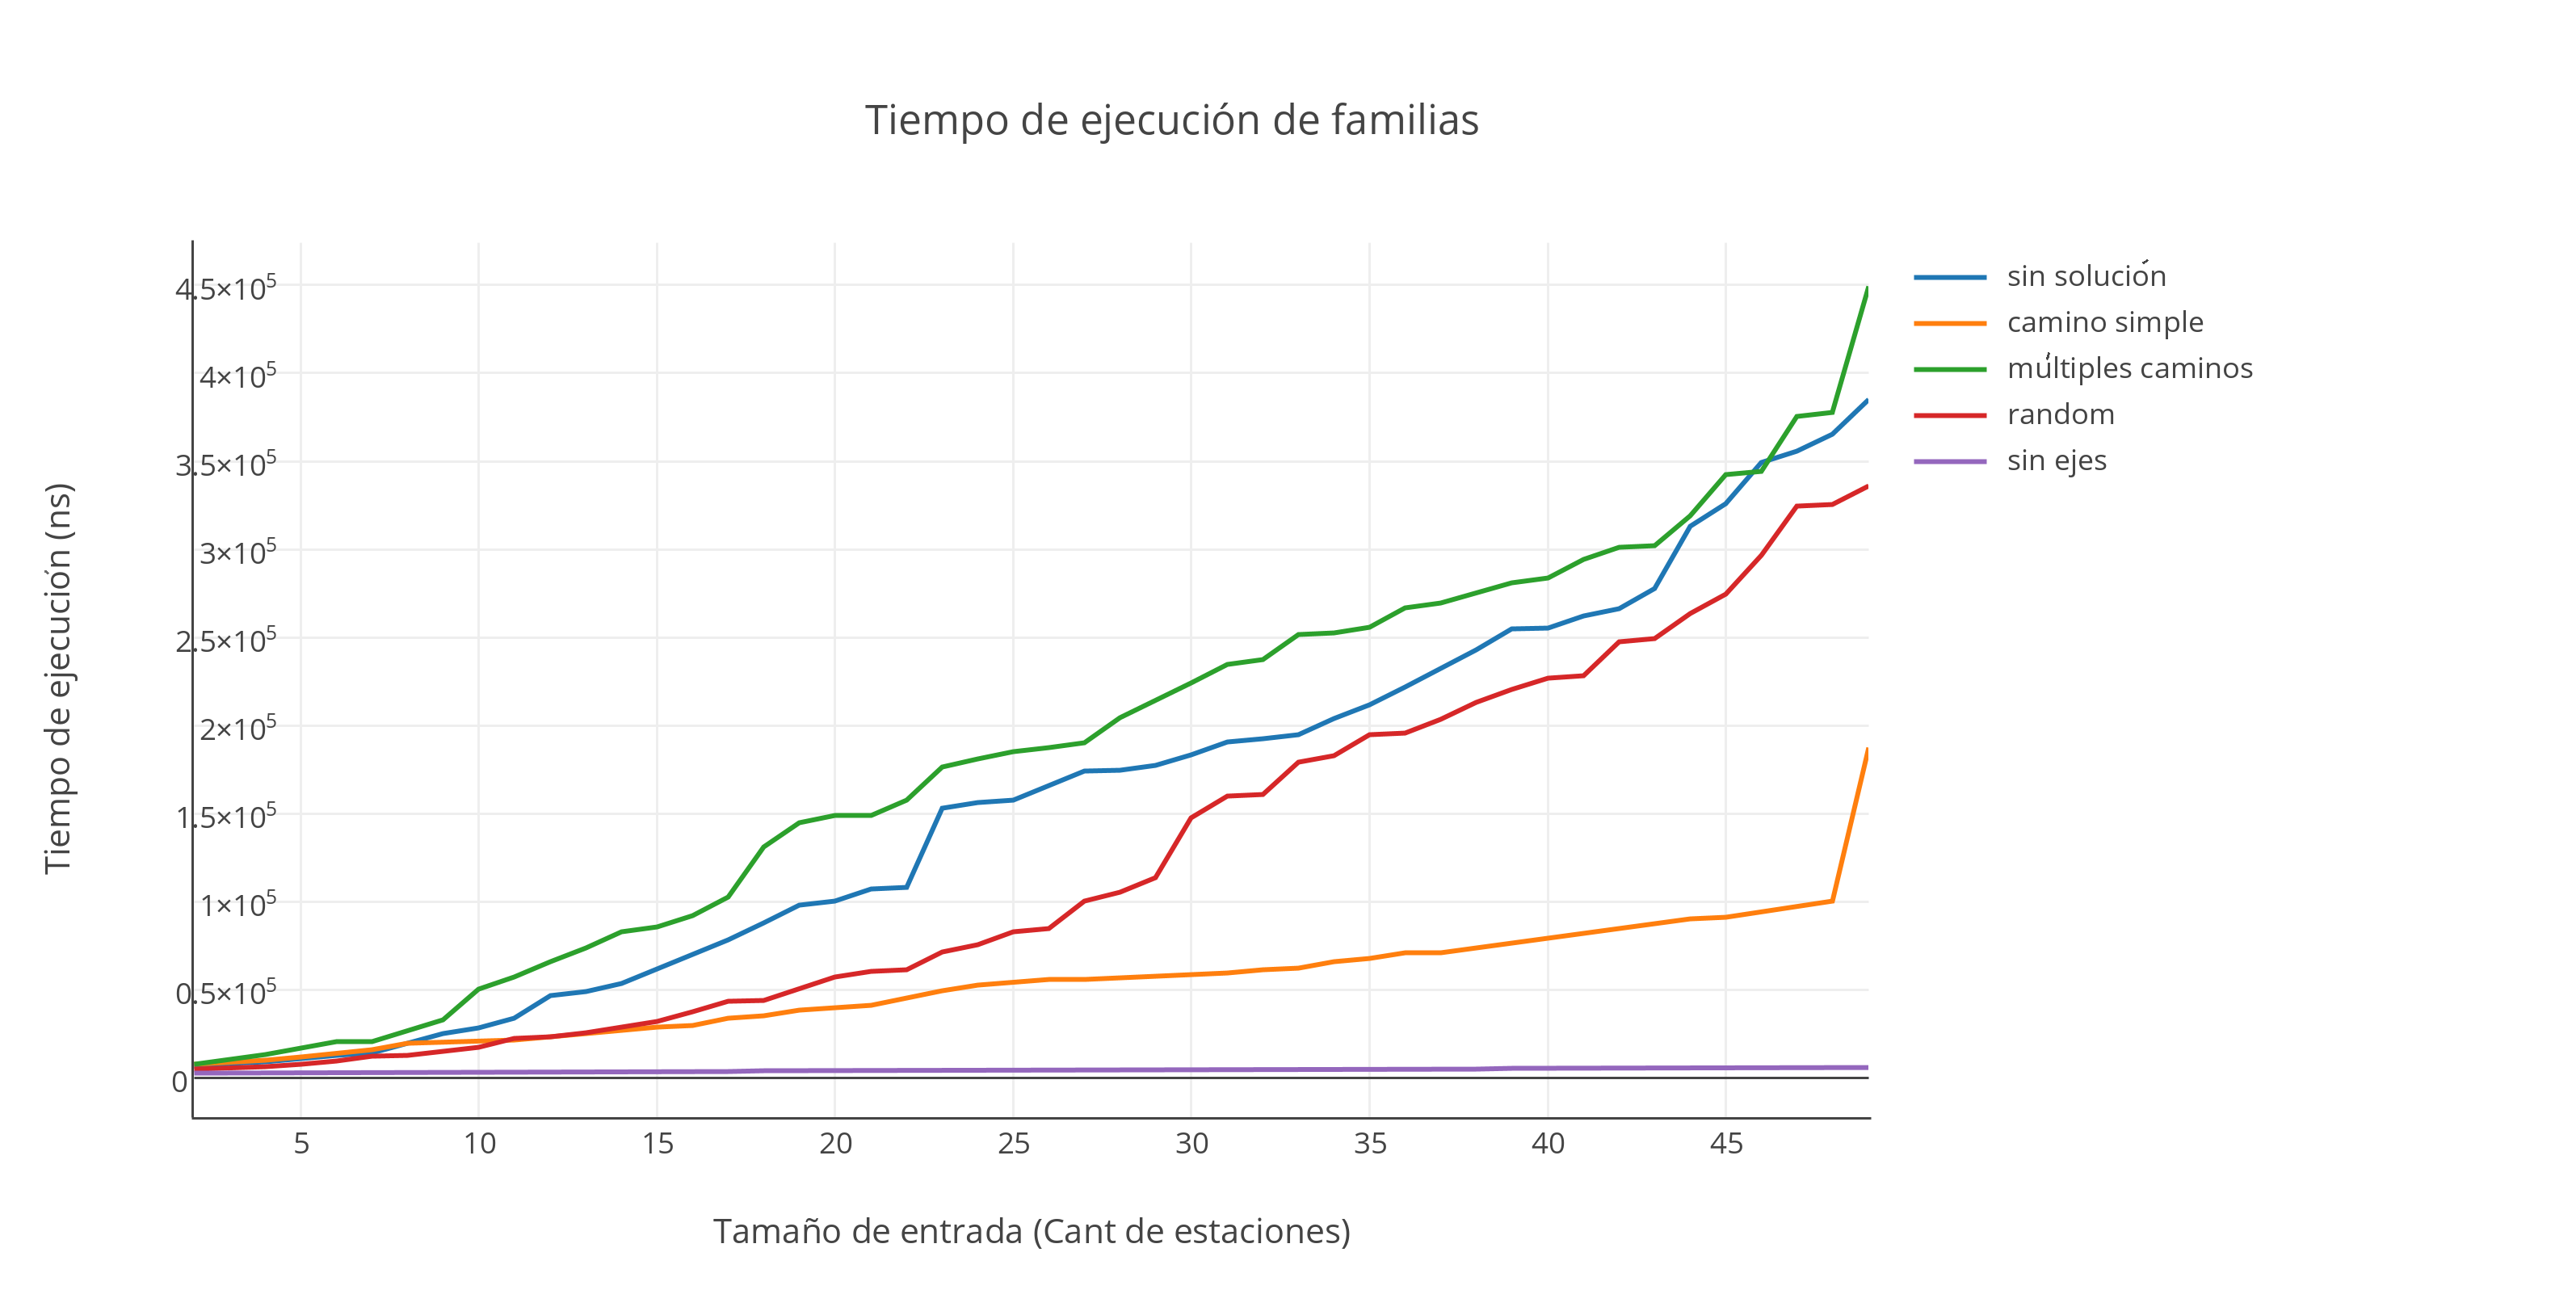
\includegraphics[scale=0.65]{./EJ3/comparativo.png}
 {$Gr$\'a$fico$ \ 3.1 - $Comparativo$}
  \end{center}
  \vspace*{0.3cm}

Como se observa en el gr\'afico la funci\'on representativa de la familia n\'umero 2, presenta una mejor performance en relaci\'on a las otras. Esto se debe a que nuestro algoritmo intenta chequear las aristas para armar los caminos y como encuentra que no hay ningun camino de ningún nodo hacia otro finaliza su ejecuci\'on demandando unicamente la creaci\'on del grafo.

Luego de chequear dichas instancias, llegamos a la conclusi\'on que la familia de casos que presenta una mejor performance para nuestro algoritmo
es la familia número 2: \textbf{Sin ejes, todos los nodos desconectados}

Un grafo representativo de lo dicho ser\'ia el siguiente:

\vspace*{0.3cm} \vspace*{0.3cm}
  \begin{center}
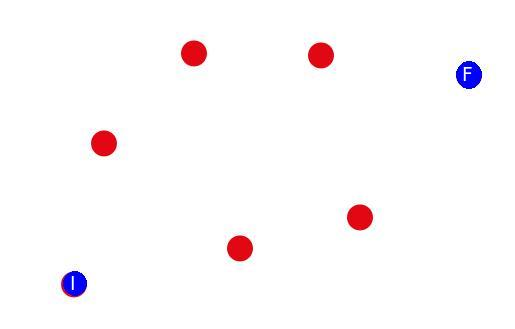
\includegraphics[scale=0.5]{./EJ3/grafoSinEjes.jpeg}
\\{$Grafo$ \ 3.1 - \textit{Mejor caso, no tiene ejes todos las estaciones estan desconectadas}} 
  \end{center}
  \vspace*{0.3cm}
  
Luego, verificando el peor caso, llegamos a la conclusi\'on que la familia de casos en el que resulta menos beneficioso trabajar con nuestro algoritmo ser\'a la familia de casos número 4: \textbf{el grafo que se obtiene de transformar el circuito de estaciones de entrada es aquel que presenta multiples caminos para llegar a destino donde la suma de estos caminos presentan el mismo valor}, dandonos el siguiente grafo:\\

\vspace*{0.3cm} \vspace*{0.3cm}
  \begin{center}
 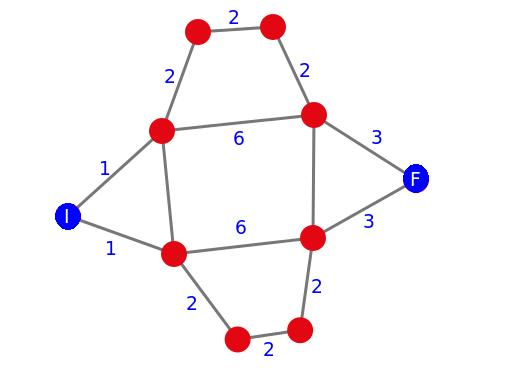
\includegraphics[scale=0.5]{./EJ3/grafoMultiCamino.jpeg}
 \\{$Grafo$ \ 3.2 - $Peor$ $Caso$}
  \end{center}
  \vspace*{0.3cm}

Veamos en detalle como se comportan el mejor y peor caso con respecto a la complejidad calculada.\\

  \vspace*{0.3cm} \vspace*{0.3cm}
  \begin{center}
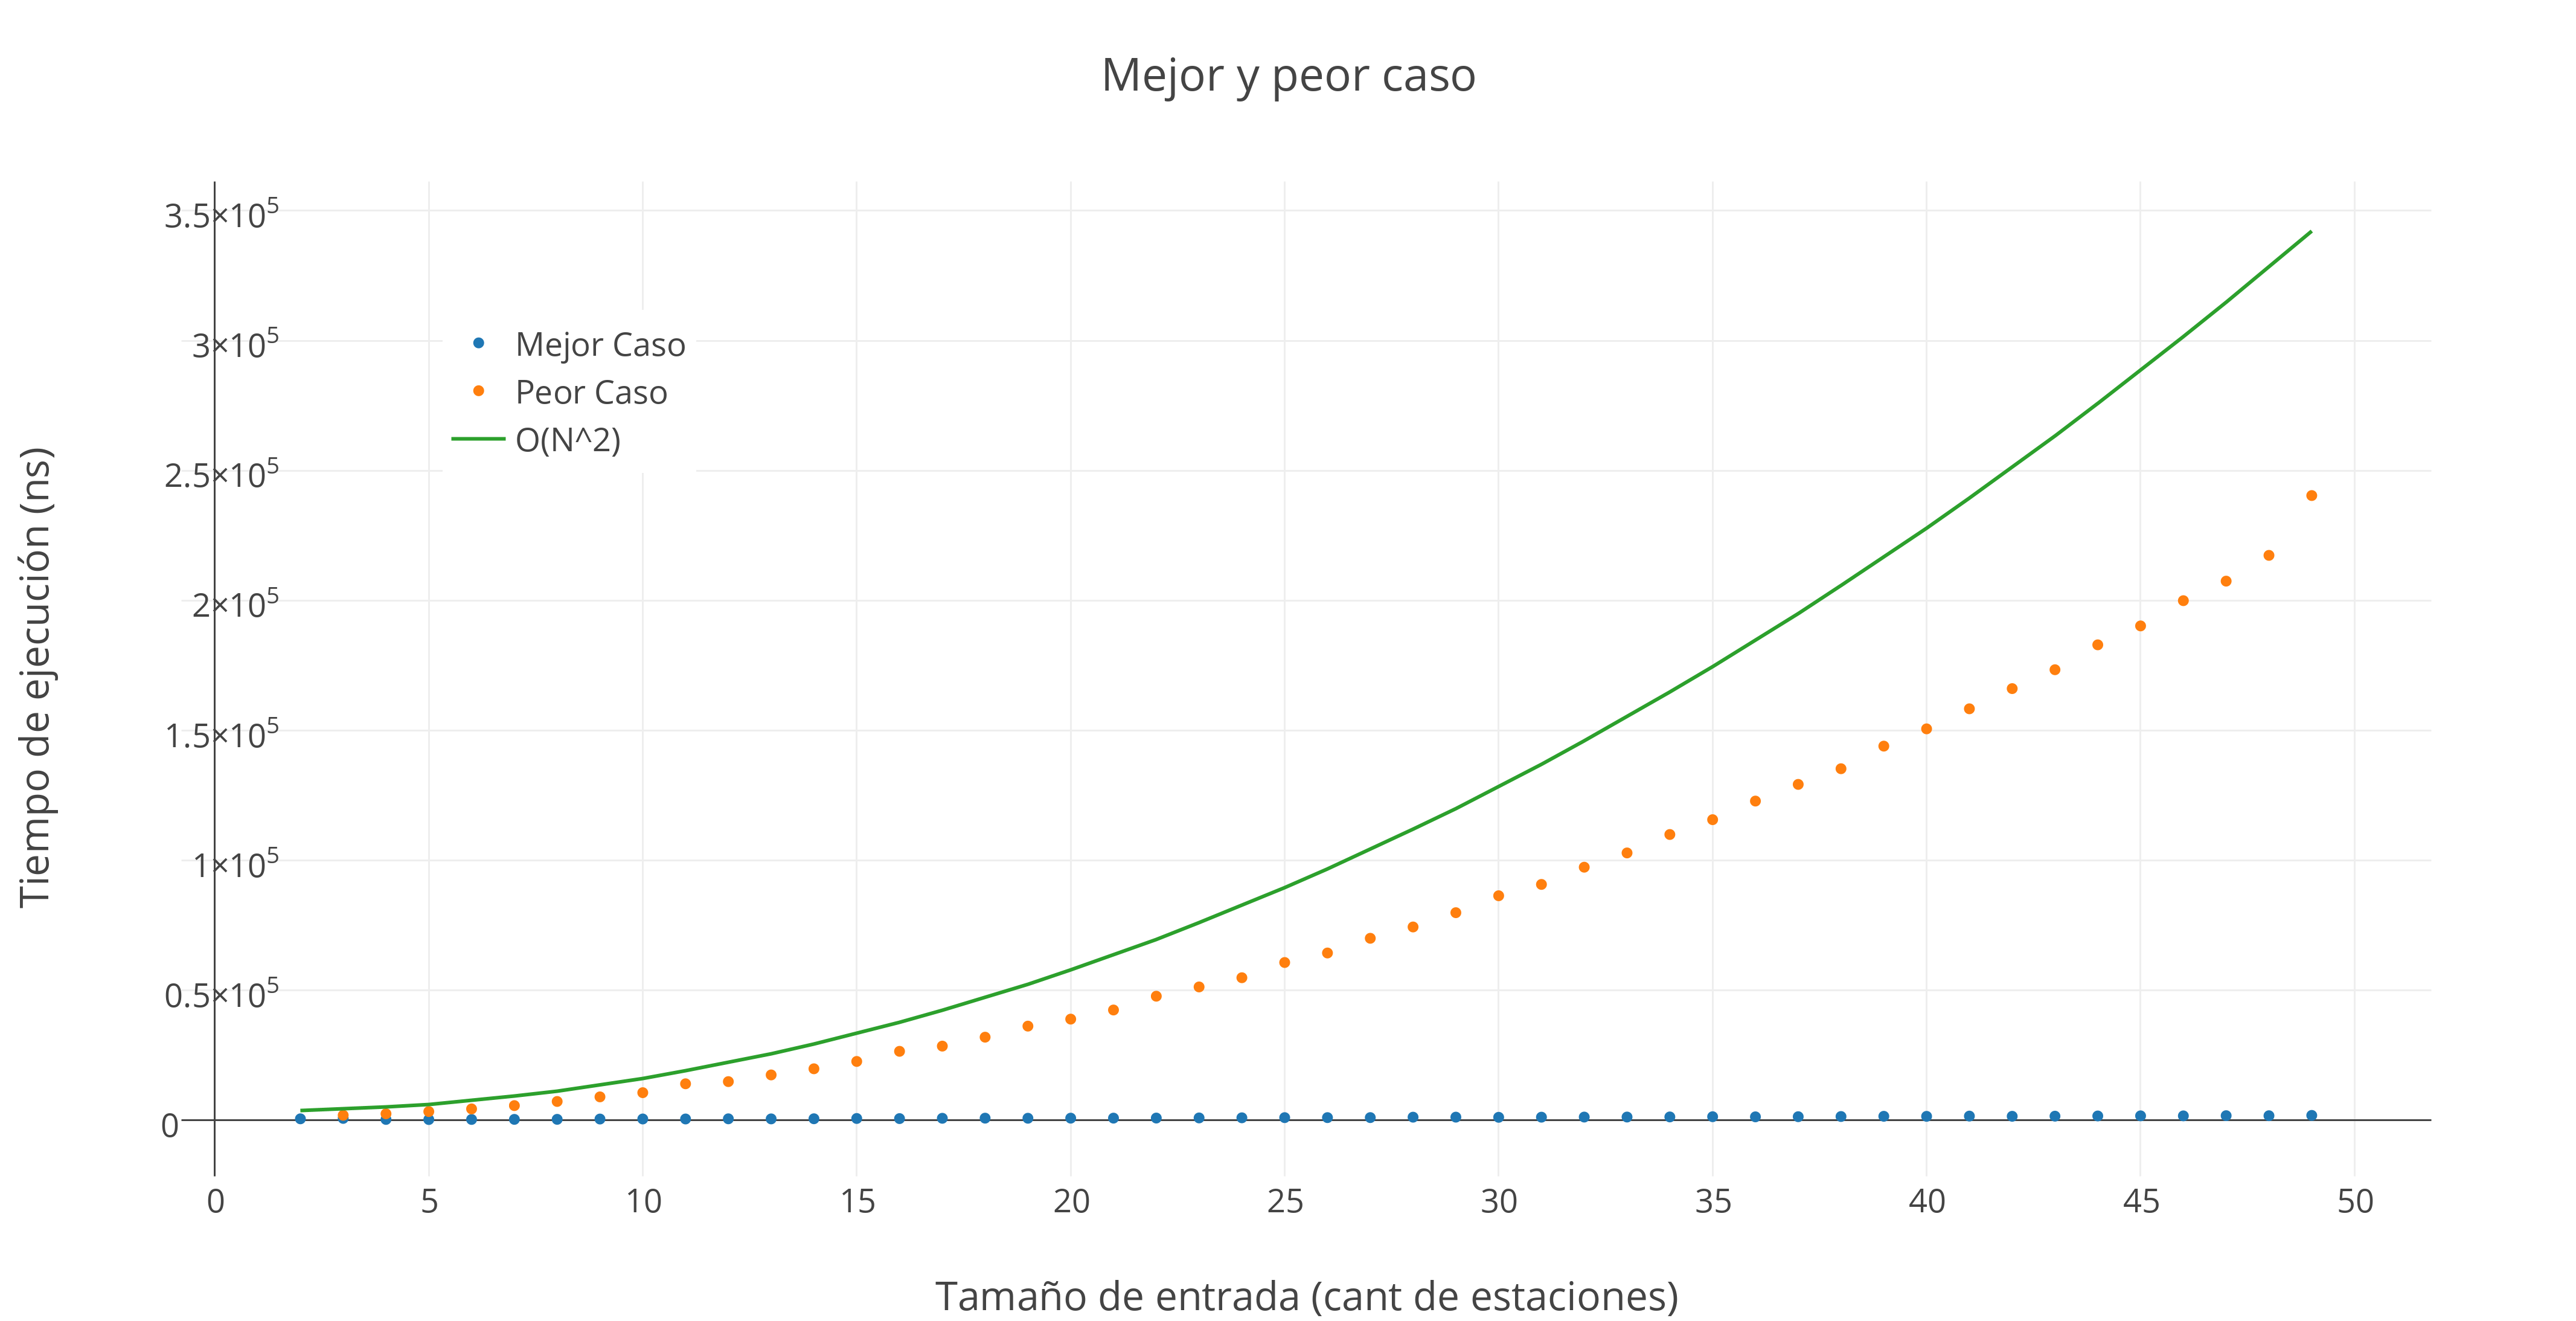
\includegraphics[scale=0.5]{./EJ3/mejorYpeorCaso.png}
{Gr\'afico 3.2 - $Comparativo$}
  \end{center}
  \vspace*{0.3cm}

Podemos ver en este gr\'afico comparativo como las familias est\'an acotadas por la funci\'on de la complejidad te\'orica calculada.\\

La cota de la complejidad fue encontrada con una aproximaci\'on mediante cuadrados m\'inimos sobre una función cuadrática, y ajustando el coeficiente principal de forma que fuese suficiente para evidenciar la pertenencia a O($N^2$).
  
Dada la escala utilizada para el gr\'afico 3.2 la función del mejor caso se torna constante, dando a entender que todas las mediciones están en cero. Es por esto que desarrollamos otro gr\'afico para poder observar con mayor detenimiento dicha funci\'on.
Además, como el mejor caso se da cuando no hay ejes, el costo total del algoritmo es O(N). Por lo tanto, mostraremos esto acotando los resultados por una función lineal que fue obtenida realizando cuadrados m\'inimos y buscando un valor adecuado para el coeficiente principal lo suficientemente grande para lograr la cota.

  \vspace*{0.3cm} \vspace*{0.3cm}
  \begin{center}
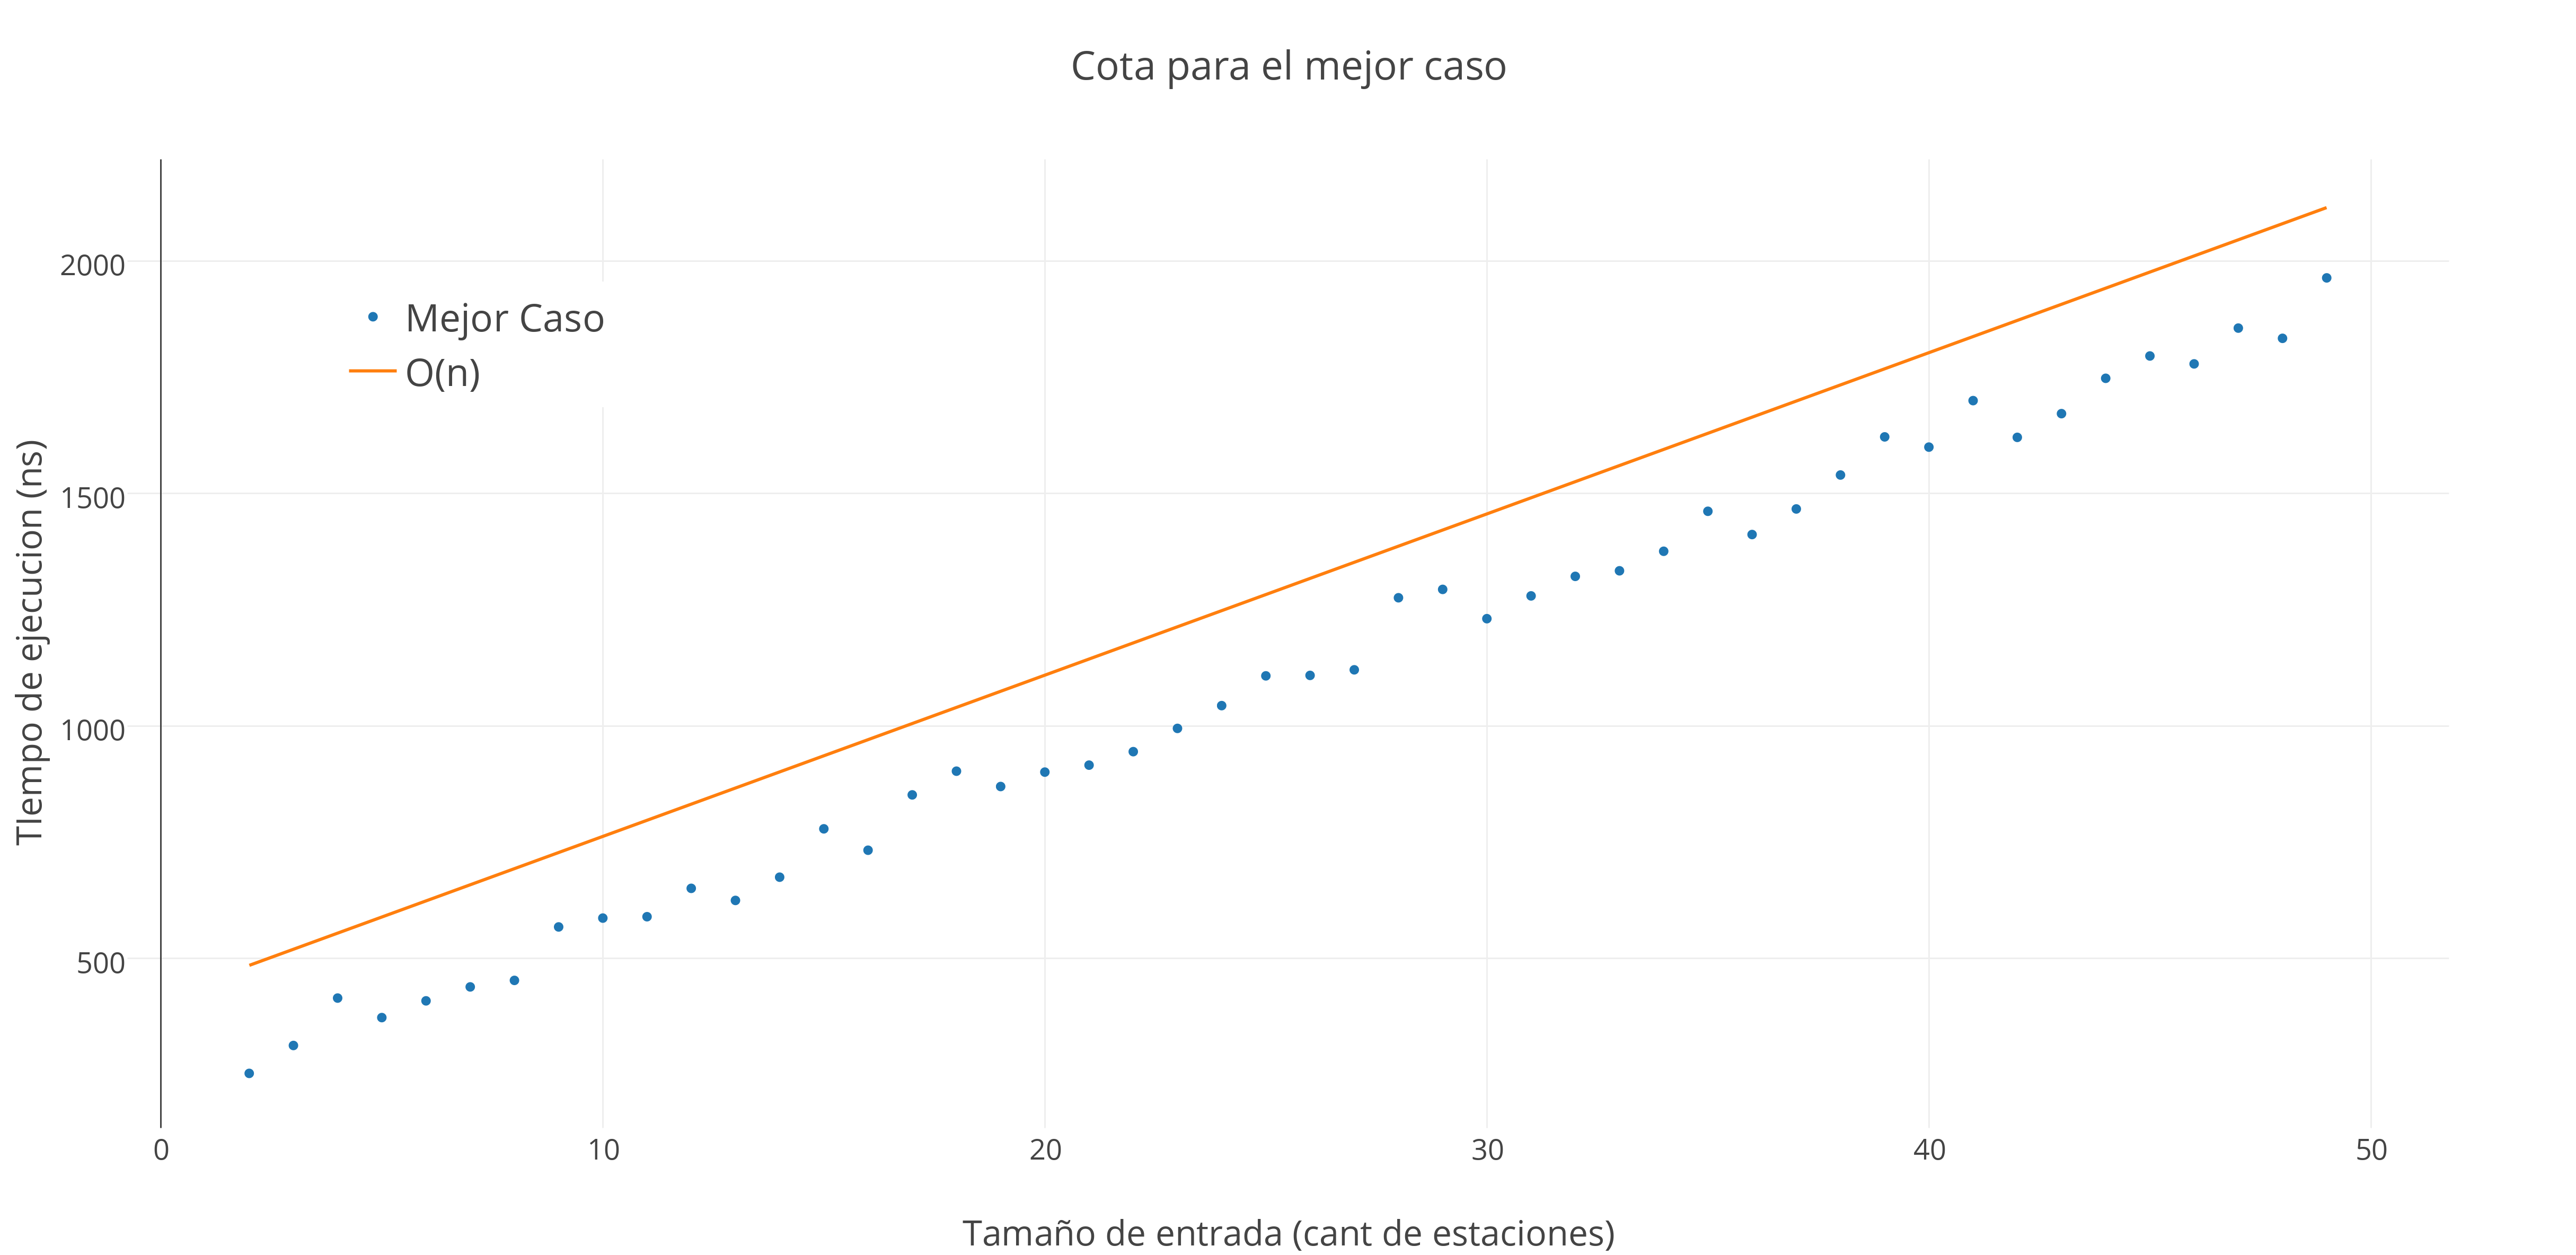
\includegraphics[scale=0.5]{./EJ3/Mejorcasoycotainferior.png}
{Gr\'afico 3.3 - \textit{Mejor caso contra cota inferior}}
  \end{center}
  \vspace*{0.3cm}

Podemos concluir luego de los tests realizados, que el algoritmo se mantiene dentro de la cota de complejidad calculada. 

Pudimos observar además, detalles relacionados al funcionamiento del algoritmo y que es lo que sucede cuando se presentan.

Concluimos finalmente, que el algoritmo resuelve el problema de las estaciones ofreciendo el mejor resultado para todos los casos.
